\documentclass[12pt]{article}

\usepackage[utf8]{inputenc}
\usepackage[spanish]{babel}

\usepackage{amssymb, amsmath}

\usepackage{geometry}
\geometry{margin=2.54cm}

\usepackage{graphicx}

\pagestyle{plain}

\begin{document}

% Portada
\begin{titlepage}
	\centering
	{\scshape\LARGE Universidad Aztlán \par}
	\vspace{1cm}
	{\scshape\Large Campus Playa del Carmen \par}
	\vspace{3cm}
	{\scshape\Huge Álgebra de Vectores \par}
	\vspace{1cm}
	{\itshape\Large Vectores en $\mathbb{R}^2$, $\mathbb{R}^3$ y su interpretación geométrica \par}
	\vspace{3cm}
	{\Large José Rosendo Camal Teh \par}
	\vfill
	{\Large Ingeniería en Sistemas Computacionales \par}
	{\Large Tercer Cuatrimestre \par}
	{\Large Cálculo Vectorial \par}
	\vfill
	{\Large Prof. Luis Alberto Garibaldi Leciwr \par}
	\vfill
	{\Large 13 de mayo de 2026 \par}
	\vfill
	{\Large Playa del Carmen, Quintana Roo \par}
\end{titlepage}

\section*{Actividades}

% Actividad 1
\subsection*{Actividad 1}

\textbf{Instrucciones:} Representar gráficamente el vector:
\[ \vec{A} = \left( 5, 2 \right) \]
y calcular su magnitud.
\newline

\textbf{Solución:}
La magnitud del vector $\vec{A}$ es igual a la raíz cuadrada de la suma de los cuadrados de sus componentes ---aplicación del Teorema de Pitágoras---:

\begin{align*}
	|\vec{A}| &= \sqrt{ (5)^2 + (2)^2 } \\
	&= \sqrt{ 25 + 4 } \\
	&= \sqrt{29} \\
	|\vec{A}| &= \sqrt{29}
\end{align*}

De esta manera, obtenemos que la magnitud de $\vec{A}$ es $\sqrt{29}$, aproximadamente igual a 5.385. A continuación, la representación gráfica del vector:

\begin{figure}[htb]
	\centering
	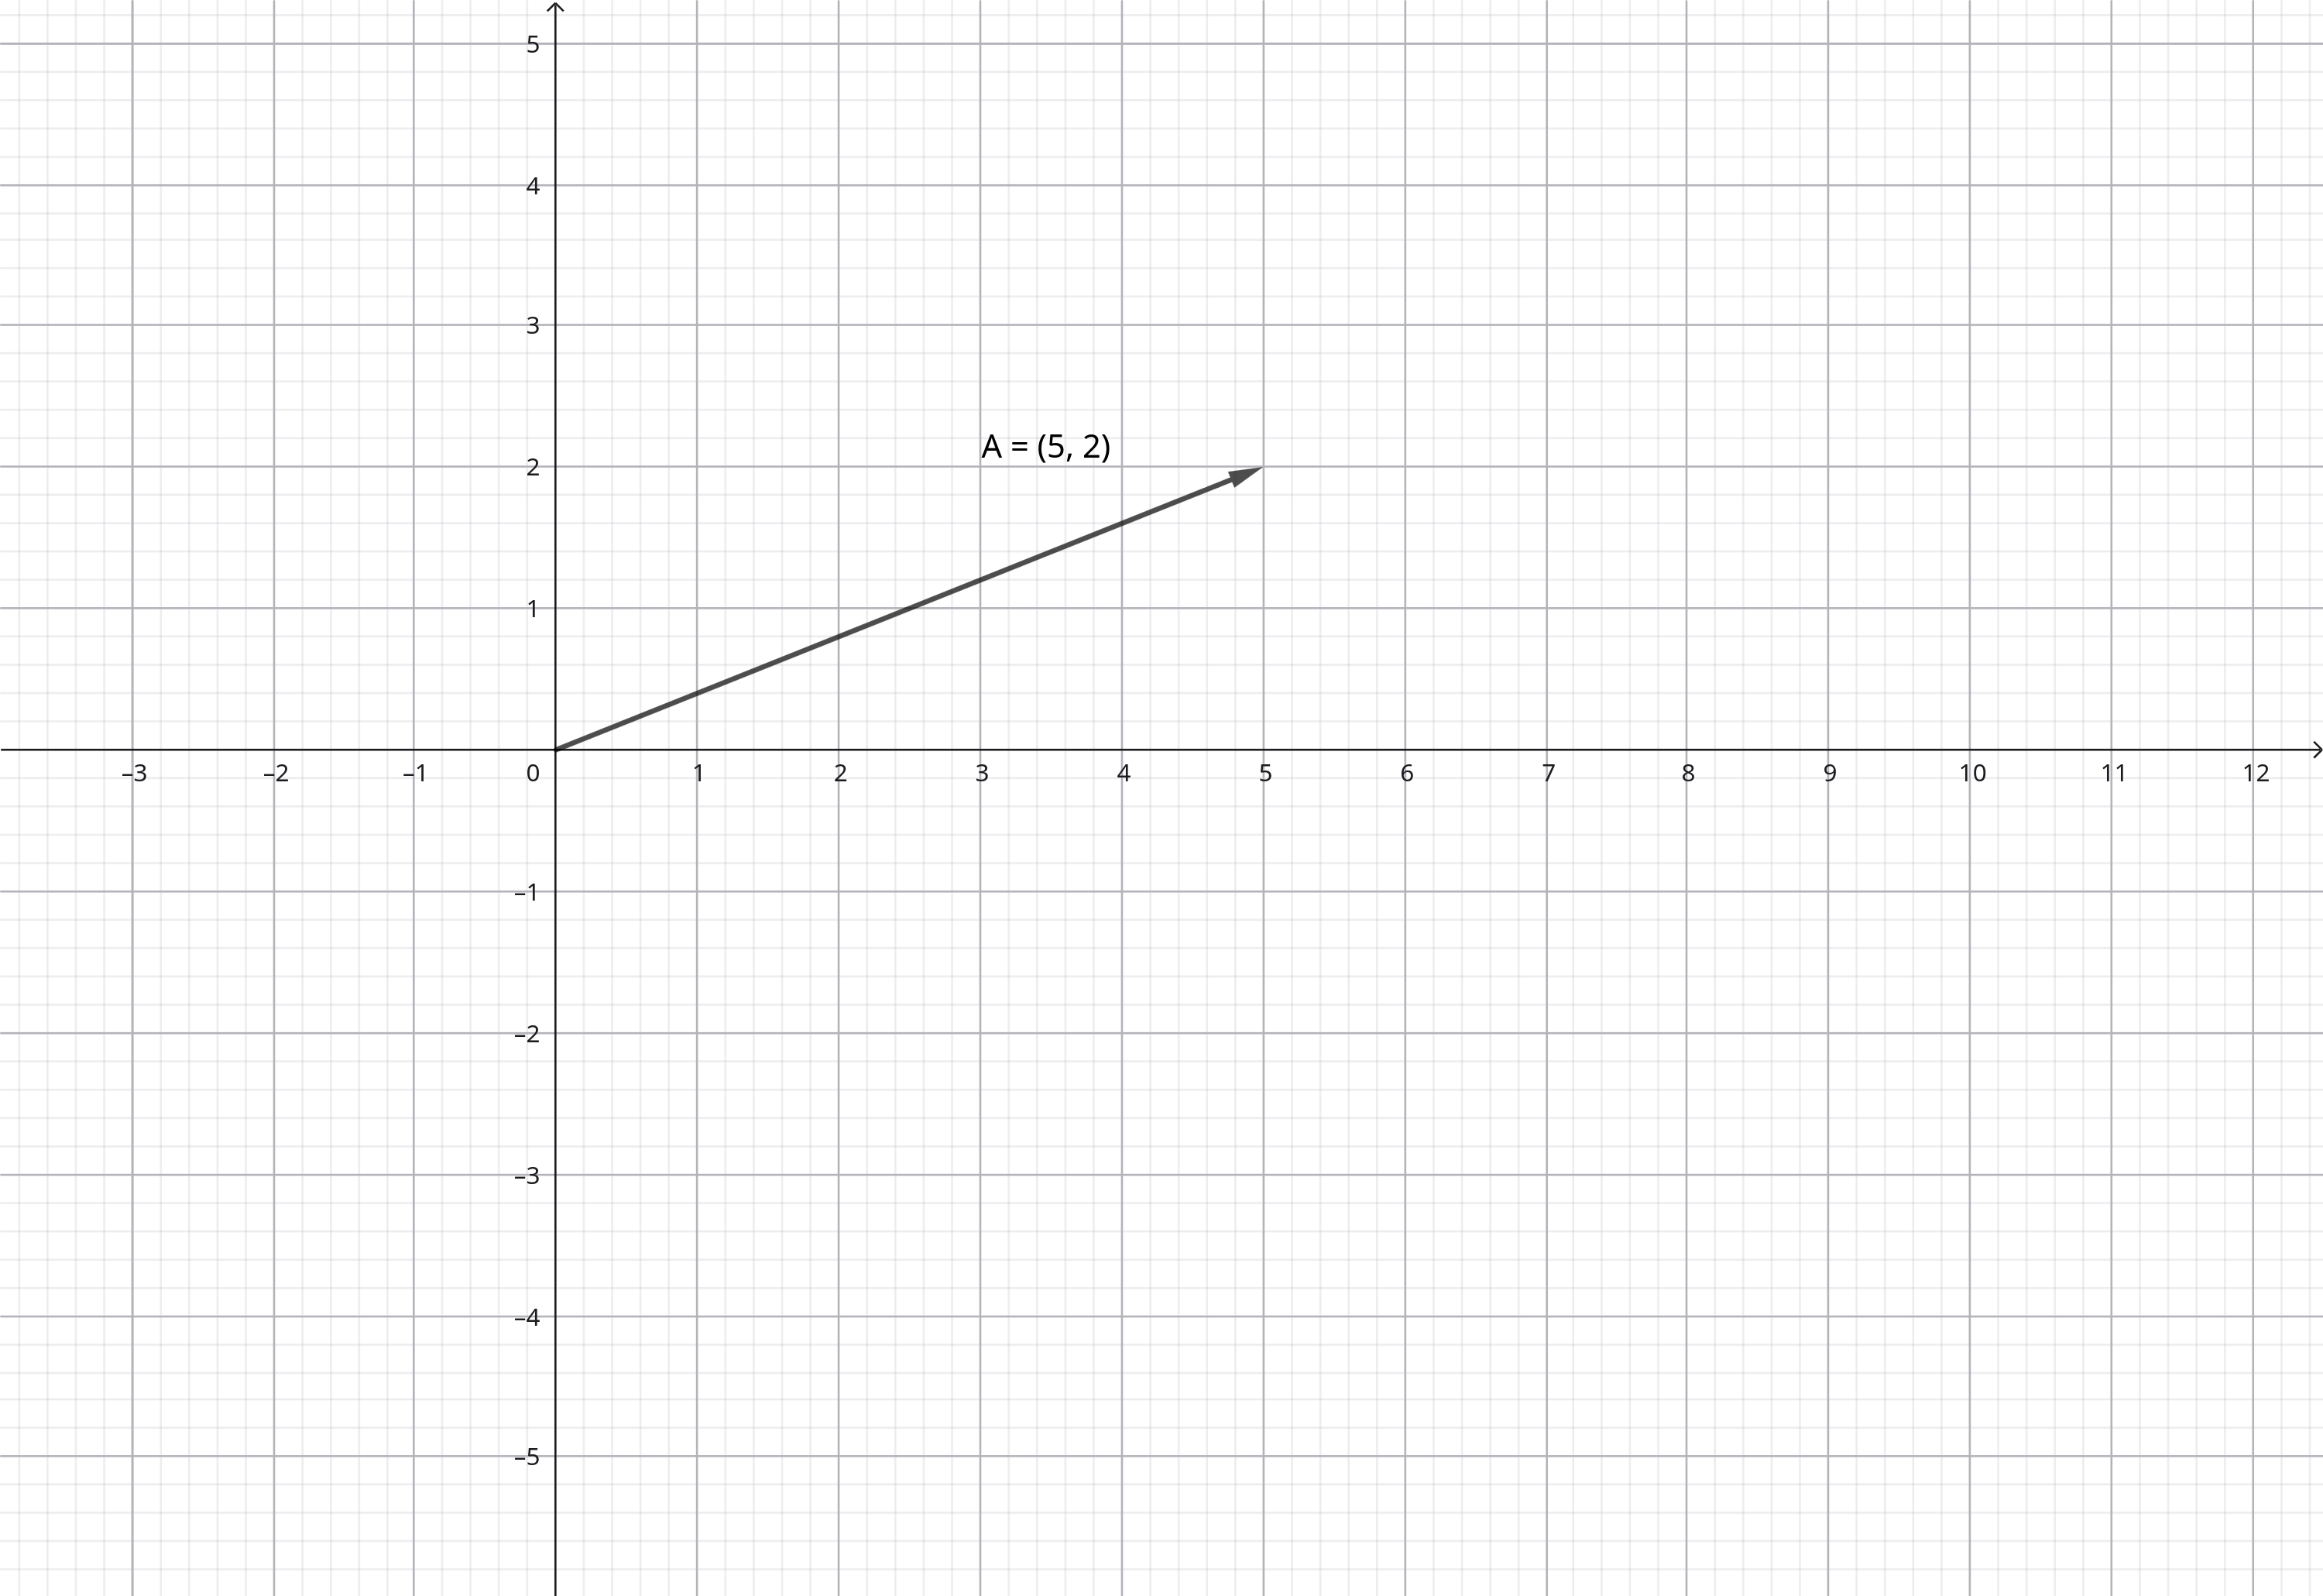
\includegraphics[scale=0.8]{geogebra-export_1.png}
\end{figure}

% Actividad 2
\subsection*{Actividad 2}

\textbf{Instrucciones:} Encuentra la magnitud del vector:
\[ \vec{B} = \left( 4, 7, 1 \right) \]

\textbf{Solución:} La magnitud $|\vec{B}|$ es:
\begin{align*}
	|\vec{B}| &= \sqrt{ (4)^2 + (7)^2 + (1)^2 } \\
	&= \sqrt{ 16 + 49 + 1 } \\
	&= \sqrt{ 16 + 50 } \\
	&= \sqrt{66} \\
	|\vec{B}| &= \sqrt{66}
\end{align*}

Dado lo anterior, la magnitud $|\vec{B}|$ es igual a $\sqrt{66}$ y esta a su vez es, aproximadamente, igual a 8.124.

% Actividad 3
\subsection*{Actividad 3}

\textbf{Instrucciones:} Un montacargas se mueve:
\begin{itemize}
	\item 8 metros hacia adelante
	\item 6 metros hacia la derecha
	\item 2 metros hacia arriba
\end{itemize}

Representar el vector y calcular su magnitud.
\newline

\textbf{Solución:}
El vector que representa el movimiento del montacargas es de la forma:
\[ \vec{M} = (x, y, z) \]
donde $x$ corresponde al movimiento hacia adelante, el componente $y$ el movimiento hacia la derecha y por último, $z$ representa el movimiento hacia arriba. De esta manera, el vector $\vec{M}$ es:
\[ \vec{M} = (8, 6, 2) \]

La magnitud de $\vec{M}$ se calcula con la raíz cuadrada de la suma de los cuadrados de los componentes:

\begin{align*}
	|\vec{M}| &= \sqrt{ (8)^2 + (6)^2 + (2)^2 } \\
	&= \sqrt{ 64 + 36 + 4 } \\
	&= \sqrt{ 64 + 40 } \\
	&= \sqrt{104} \\
	&= \sqrt{2 \left( 52 \right) } \\
	&= \sqrt{2 \cdot 2 \cdot 26} \\
	&= 2\sqrt{26} \\
	|\vec{M}| &= 2 \sqrt{26}
\end{align*}

Dado lo anterior, la magnitud del vector $\vec{M}$ es $2\sqrt{26} \approx$ 10.19.
\end{document}

